\documentclass[tikz]{standalone} % Declare standalone class, enable TikZ options
\usepackage{tikz} % Load the TikZ package
\usetikzlibrary{shapes.geometric} % Example: Load a TikZ library

\begin{document} % Begin the document

% \begin{tikzpicture}
%         \def\firstcircle{(-.5,0) circle (2.65cm)}
%         \def\secondcircle{(2.5,0) circle (2.65cm)}
        
%         % Fill the symmetric difference
%         \fill[even odd rule, gray]\firstcircle \secondcircle;
        
%         % Draw the circle outlines and add labels
%         \draw[draw=black,line width=.75mm] \firstcircle;
%         \draw[draw = black, line width=.75mm] \secondcircle;
%         \node at (-3.3,1.9) {\Large$A$};
%         \node at (5.3,1.9) {\Large$B$};
%     \end{tikzpicture}

    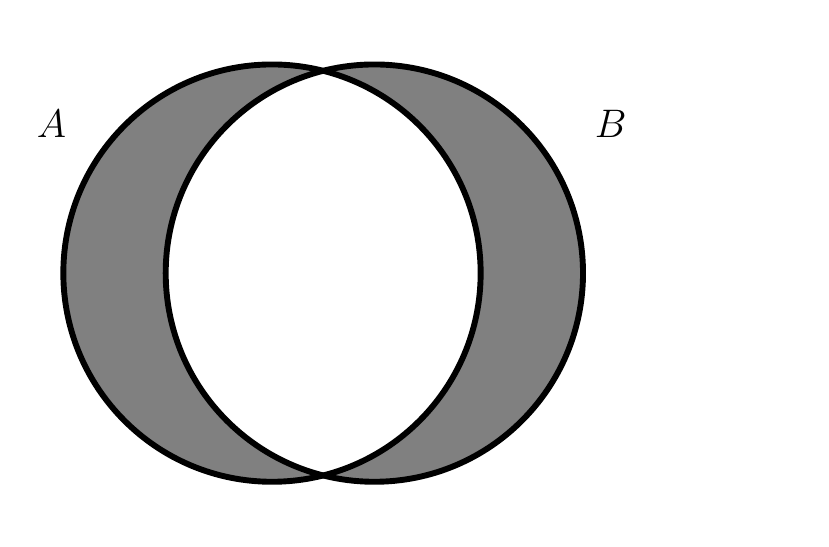
\begin{tikzpicture}
        \def\firstcircle{(-.5,0) circle (2.65cm)}
        \def\secondcircle{(.8,0) circle (2.65cm)}
        
        % Fill the symmetric difference
        \fill[even odd rule, gray]\firstcircle \secondcircle;
        
        % Draw the circle outlines and add labels
        \draw[draw=black,line width=.75mm] \firstcircle;
        \draw[draw = black, line width=.75mm] \secondcircle;
        \node at (-3.3,1.9) {\Large$A$};
        \node at (3.8,1.9) {\Large$B$};
        \node at (6.1,3) {};
        \node at (6.1,-3) {};
    \end{tikzpicture}

    % \begin{tikzpicture}
    %     \def\firstcircle{(-.5,0) circle (2.65cm)}
    %     \def\secondcircle{(3.5,0) circle (2.65cm)}
        
    %     % Fill the symmetric difference
    %     \fill[even odd rule, gray]\firstcircle \secondcircle;
        
    %     % Draw the circle outlines and add labels
    %     \draw[draw=black,line width=.75mm] \firstcircle;
    %     \draw[draw = black, line width=.75mm] \secondcircle;
    %     \node at (-3.3,1.9) {\Large$A$};
    %     \node at (6.1,1.9) {\Large$B$};
    %     \node at (6.1,3) {};
    %     \node at (6.1,-3) {};
    % \end{tikzpicture}
   

\end{document} % End the document